\newpage
\subsection{Coastal sea level signal from a 0.1 degree B-grid \OGCM{}}
\label{S:plan_whichcell}
\subsubsection{Problem and motivation}

% intro
Although nominally a blue-water forecasting system, the representation of coastal phenomena in \BL{} has become a topic of increasing operational interest.\\
Initially, this interest was restricted to visual inspection of forecast daily average SLA maps; an  output configuration reflecting the systems target of mesoscale eddies.   Subsequent quantitative assessment \citep{Taylor:2010ud} has been restricted to observations from coastal tide gauges.  Tide gauges being essentially the only observation platform available for routine sea level skill evaluation \BL{}.\\



% setup current evaluation
After several years of maturing interest it is now relevant to re-evaluate exactly how to map the gridded model output to insitu coastal locations. This is a non-trivial matter at the cross-over of representational limits of both the model and observations.\\
Fundamental to this problem is that geographic locations of tide gauges do not coincide exactly with the coastal boundary of the \OGCM{}.  The numerical coast is a key discontinuity represented by a land/sea mask in gridded space.  
\BoxBegin{}
Given that \BL{} uses a staggered Arakawa B-grid at 0.1 degree spacing, can the output be meaningfully mapped to real coastal locations and with what limitations? Is extrapolation valid and why?\\
\BoxEnd{}
All comparisons made to date have utilised a 'nearest coastal neighbour' approach; a choice to directly map the tide gauge location to the geographically closest tracer cell adjacent to the models land/sea interface.  



Closer inspection of the \BL{} configuration has brought certain aspects of model to the fore that invite reconsideration of the 'nearest closest neighbour' approach, namely;
\begin{inparaenum}[(a)]
\item numerics of lateral boundary conditions;
\item split explicit solver scheme;
\item smoothing and suppression of the b-grid checkerboard null mode.
\end{inparaenum}
In addition, since the earlier studies, access to tide gauge data has expanded and recent configurations of \BL{} have provided higher temporal frequency outputs (now 3 hourly averages).\\


\begin{figure}[!h]
	\centering
%	\subfloat[Illustration of Arakawa B-grid overlaid on the coastline represented (black).  Sea level is located at `T' cells whereas velocity is at the staggered `U' cells.  Geographic tide gauge locations can fall beyond the nominal spatial coverage of the model ocean.]{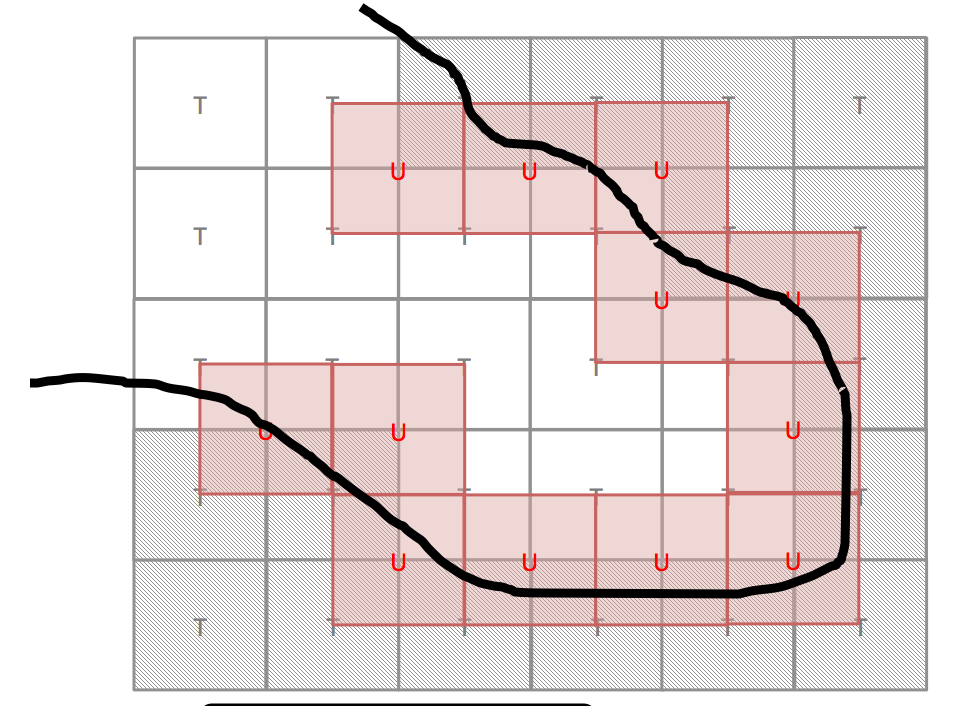
\includegraphics[width=80mm]{figures_3/coastal_masking.png}}\\
	\subfloat[Spatial extent of \OGCM{} T-cells and location of two coastal tide gauges; the possible correspondence of modeled and observed sea level must be subject to limitations]{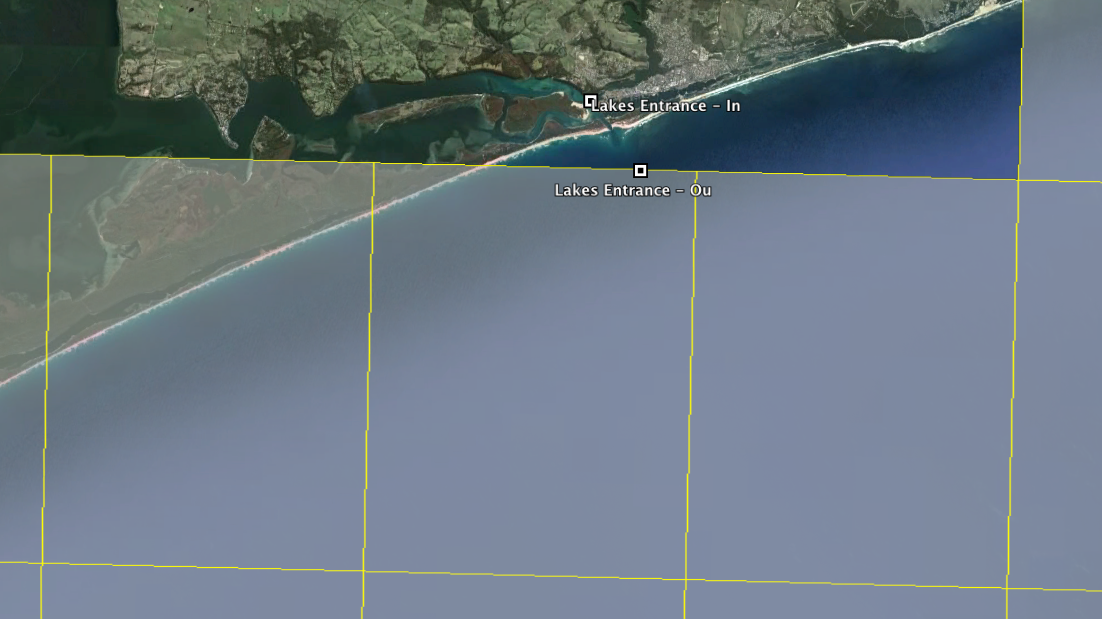
\includegraphics[width=110mm]{figures_3/OFAM_lakes_entrance.png}}\\

	\subfloat[\MOM{} numerical stencils of notable relevance to grid scale noise]{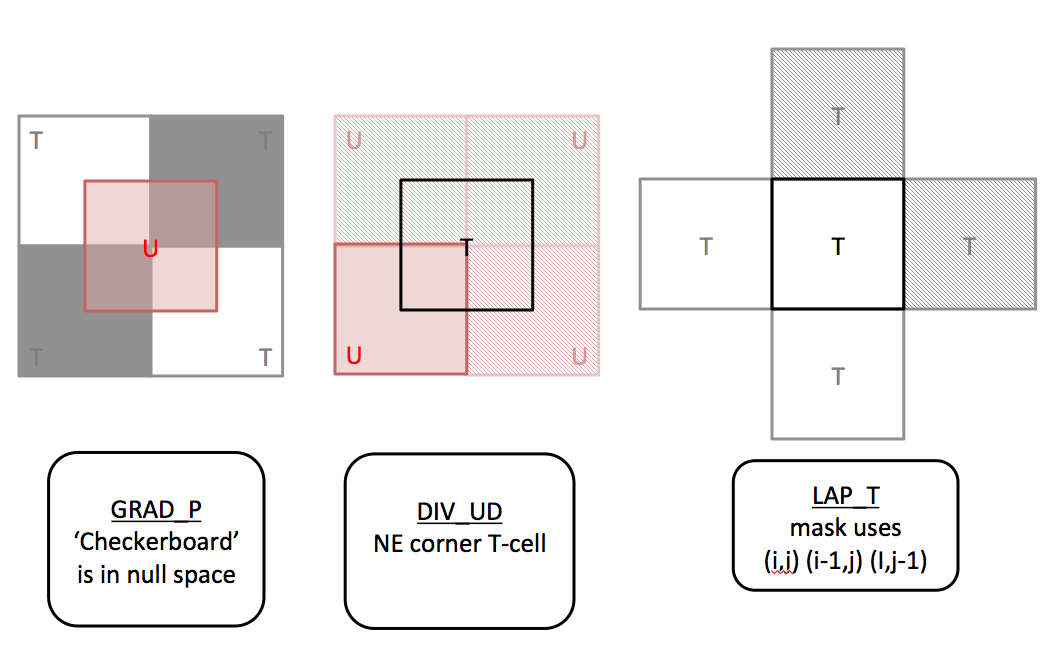
\includegraphics[width=100mm]{figures_3/mom_BT_stencils_extra.png}}
	%\caption{}
	\label{fig:cells_coast}
\end{figure}

\subsubsection{Data sources}
Attention will be restricted to \BL{} behind real time analysis data - so as to set aside questions of forecast skill and focus on spatial representation.\\
Operational output from a neighbourhood about each nominal location will be extracted for the history of the present operational version. \\
Observations will be taken from a subset of those tide gauges that routinely stream data to the \BOM{} (or have the potential to).



\subsubsection{Method outlook}
Primarily this investigation is an empirical comparison of tide gauges observations to a neighbourhood of grid cells.\\
A subset of focus locations will be chosen to specifically explore questions of B-grid noise and the effects of unresolved embayments.   This subset will include: Outer Harbour in SA and Port Phillip Bay in Vic.\\  
Guided by an exposition of relevant numerical operators, a series of mapping methods will be empirically evaluated.   Ultimately this study aims to recommend the single best method for sea level forecast aggregation.




%analytical discussion - BCs, scales, \\
%empirical evaluation:
%nearest any\\
%nearest coastal\\
%weighted combo\\
%filtered ... 
